% 
% Lecture Template for ME3050 -  Dynamics Modeling and Controls - Tennessee Technological University
%
% Spring 2020 - Summer 2020
% Tristan Hill, May 07, 2020
% Module 3 - Energy Methods
% Topic 1 - 
%

\documentclass{beamer}                         % for presentation (has nav buttons at bottom)
%\documentclass[handout]{beamer}  % for handout 
\usepackage{beamerthemesplit}
\usepackage{amsmath}
\usepackage{listings}
\usepackage{multicol}
\usepackage{framed}

\beamertemplateballitem

% custom colors
\definecolor{TTUpurple}{rgb}{0.3098, 0.1607, 0.5176} % TTU Purple (primary)
\definecolor{TTUgold}{rgb}{1.0000, 0.8666, 0.0000} % TTU Gold (primary) 
\definecolor{mygray}{rgb}{.6, .6, .6}
\definecolor{mypurple}{rgb}{0.6,0.1961,0.8}
\definecolor{mybrown}{rgb}{0.5451,0.2706,0.0745}
\definecolor{mygreen}{rgb}{0, .39, 0}
\definecolor{mypink}{rgb}{0.9960, 0, 0.9960}

% color commands
\newcommand{\R}{\color{red}}
\newcommand{\B}{\color{blue}}
\newcommand{\BR}{\color{mybrown}}
\newcommand{\K}{\color{black}}
\newcommand{\G}{\color{mygreen}}
\newcommand{\PR}{\color{mypurple}}
\newcommand{\PN}{\color{mypink}}
\newcommand{\OR}{\color{TTU}}
\newcommand{\GD}{\color{TTUgold}}


\setbeamercolor{palette primary}{bg=TTUpurple,fg=TTUgold}
\setbeamercolor{palette secondary}{bg=black,fg=TTUgold}
\setbeamercolor{palette tertiary}{bg=black,fg=TTUpurple}
\setbeamercolor{palette quaternary}{bg=TTUgold,fg=black}
\setbeamercolor{structure}{fg=TTUpurple} % itemize, enumerate, etc
\setbeamercolor{section in toc}{fg=TTUpurple} % TOC sections

%\usefonttheme{professionalfonts}

\newcommand{\LNUM}{3\hspace{2mm}} % Lecture Number 

\newcommand{\Lagr}{\mathcal{L}} % lagrangian

\newcommand{\hspcu}{\underline{\hspace{20mm}}} % large horizontal space w underline
\newcommand{\vspccc}{\vspace{6mm}\\} % large vertical space
\newcommand{\vspcc}{\vspace{4mm}\\}   % medium vertical space
\newcommand{\vspc}{\vspace{2mm}\\}     % small vertical space

\newcommand{\hspcccc}{\hspace{10mm}} % large horizontal space
\newcommand{\hspccc}{\hspace{6mm}} % large horizontal space
\newcommand{\hspcc}{\hspace{4mm}}   % medium horizontal space
\newcommand{\hspc}{\hspace{2mm}}     % small horizontal space

\author{ME3050 - Dynamics Modeling and Controls} % original formatting from Mike Renfro, September 21, 2004

\newcommand{\MNUM}{4\hspace{2mm}} % Module number
\newcommand{\TNUM}{1\hspace{2mm}} % Topic number 
\newcommand{\moduletitle}{Energy Methods }
\newcommand{\topictitle}{The Conservation of Energy} 

\newcommand{\sectiontitleI}{Brief History}
\newcommand{\sectiontitleII}{Second Law Derivation}
\newcommand{\sectiontitleIII}{Non-Conservatve Forces}
\newcommand{\sectiontitleIV}{Engineering Applications}

% custom box
\newsavebox{\mybox}

\title{Module \MNUM - \moduletitle}

\date{Mechanical Engineering\vspc Tennessee Technological University}

\begin{document}

\lstset{language=MATLAB,basicstyle=\ttfamily\small,showstringspaces=false}

\frame{\titlepage \center\begin{framed}\Large \textbf{Topic \TNUM - \topictitle}\end{framed} \vspace{5mm}}

% Section 0: Outline
\frame{

\large \textbf{Topic \TNUM - \topictitle} \vspace{3mm}\\

\begin{multicols}{2}
\begin{itemize}
	\item \sectiontitleI		\vspc % Section I
	\item \sectiontitleII 	\vspc % Section II
	\item \sectiontitleIII 	\vspc %Section III
	\item \sectiontitleIV 	\vspc %Section IV
\end{itemize}
%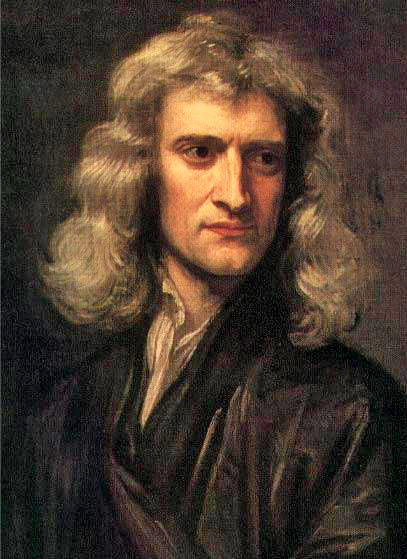
\includegraphics[scale=.25]{newton_portrait.jpg}

\end{multicols}

}

% Section I:
\section{\sectiontitleI}

\frame{
\frametitle{\sectiontitleI}

\begin{multicols}{2}
... the law of conservation of energy states that the total energy of an isolated system remains constant; it is said to be conserved over time. This law, first proposed and tested by \'{E}milie du Ch\^{a}telet, means that energy can neither be created nor destroyed; rather, it can only be transformed or transferred from one form to another.

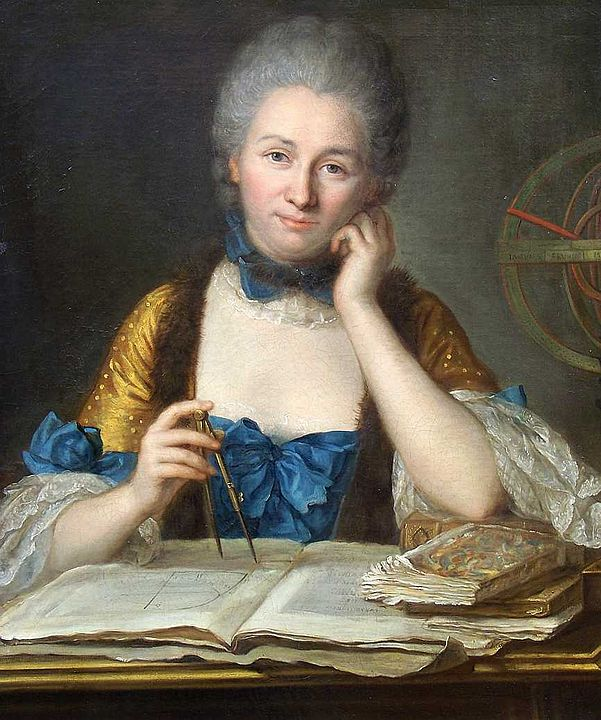
\includegraphics[scale=.25]{Emilie_Chatelet.jpg}
\end{multicols}

\vspace{5mm}
{\tiny Text: \href{https://en.wikipedia.org/wiki/Conservation_of_energy}{Wikipedia}, Image: \href{https://en.wikipedia.org/wiki/\%C3\%89milie_du_Ch\%C3\%A2telet }{Wikipedia} }

}

\frame{
\frametitle{\sectiontitleI}

\begin{multicols}{2}
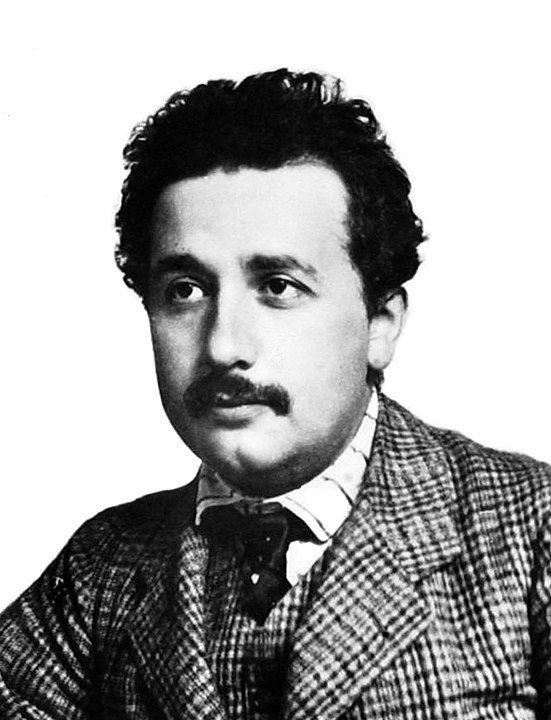
\includegraphics[scale=.22]{young_Einstein.jpg} \vspcc
{\tiny Text: \href{https://en.wikipedia.org/wiki/Conservation_of_energy}{Wikipedia} }

... however, special relativity showed that mass is related to energy and vice 
versa by $E = mc^2$, and science now takes the view that mass–energy as a 
whole is conserved. Theoretically, this implies that any object with mass can 
itself be converted to pure energy, and vice versa, though this is believed 
to be possible only under the most extreme of physical conditions ...

\end{multicols}

%\vspace{5mm}
%{\tiny Text: \href{https://en.wikipedia.org/wiki/Conservation_of_energy}{Wikipedia} }

}

% Section II:
\section{\sectiontitleII}

\frame{
\frametitle{\sectiontitleII}



A mass moves in the x direction with only the force of gravity acting on it. Netwon's Second Law combined with the definition of differential work done  by a force through a distance gives a relation between kinetic energy and work done by the external force.

\begin{multicols}{2}

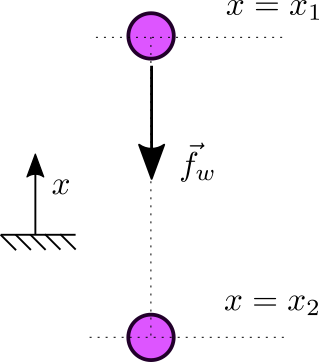
\includegraphics[scale=.4]{conservation_energy_fig1.png}

\scalebox{0.8}{${\bf f}=m{\bf a}=m\frac{d {\bf v}}{dt}$} \vspace{1mm}\\
\scalebox{0.8}{$dW={\bf f}d{\bf x}$}\vspace{1mm}\\
\scalebox{0.8}{$dW={\bf f}d{\bf x}=m{\bf a}d{\bf x}=md{\bf v}\frac{d{\bf x}}{dt}=md{\bf v}{\bf v}$}\vspace{1mm}\\
\scalebox{0.8}{$\rightarrow dW=mv_xdv_x$}\vspace{1mm}\\
\scalebox{0.8}{$W_{12}=\int_{x_1}^{x_2} mv_xdv_x=\frac{1}{2}mv_x^2|_{x_1}^{x_2}$}\vspace{3mm}\\
\scalebox{0.90}{$W_{12}=\frac{1}{2}mv_{x_2}^2-\frac{1}{2}mv_{x_1}^2=KE_1-KE_2$}

\end{multicols}

}

\frame{
\frametitle{\sectiontitleII}

Alternativley, subsitute the distance traveled into the differential work relation. Now you are left with the familar relation between work done by gravity and the potential energy in the system. 

\begin{multicols}{2}

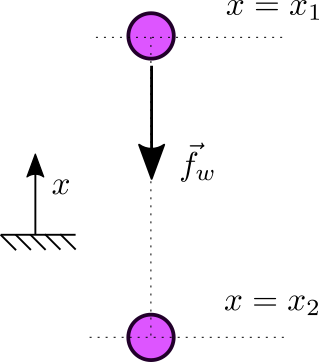
\includegraphics[scale=.35]{conservation_energy_fig1.png}

\scalebox{0.8}{$dW={\bf f}d{\bf x}$}\vspace{1mm}\\
\scalebox{0.8}{$W_{12}=\int_{x_1}^{x_2}{\bf f}d{\bf x}=(-mg)|_{x_1}^{x_2}=(-mg)(x_2-x_1)$}\vspace{1mm}\\
\scalebox{0.8}{$W_{12}=-mg(x_2-x_1)$}\vspc

Now we can see that \vspace{1mm}\\

\scalebox{0.8}{$W_{12}=-mg(x_2-x_1)=\frac{1}{2}mv_{x_2}^2-\frac{1}{2}mv_{x_1}^2$}\vspc

\scalebox{0.8}{$ \Delta KE +\Delta PE = 0 $}

\end{multicols}


}

% Section III:
\section{\sectiontitleIII}

\frame{
\frametitle{\sectiontitleIII}


}

% Section IV:
\section{\sectiontitleIV}

\frame{
\frametitle{\sectiontitleIV}


}
	
\end{document}





